\chapter{Conclusion}
%
\label{sec:conclusion}

The main focus in contemporary rendering research are non-deterministic methods for light transport simulation. Boosting the convergence of these methods is the main thrust of todays efforts in research groups world wide. In particular path-guiding based approaches are becoming increasingly popular as they have shown to improve non-deterministic methods significantly by using a global approximation of the radiance field to allow better informed decisions during stochastic sampling.

At the same time a shift in compute hardware manufacturing from clock frequency growth to growth in core count with the next generation of multi-core and many-core hardware on the horizon is seen. High performance computing centers, which have large scale multi-core parallelization at the core of their business, are opening up and undergo a transformation towards becoming providers for public massive multi-core cloud computing. Developing algorithms which cater to the characteristics of this new hardware is deemed as one of the major challenges in future rendering research.

Both trends, path-guiding and multi-core hardware, are the main motivation for revisiting deterministic methods for light transport simulation, which have received little attention in the past years. In particular there is a large body of research related to deterministic methods in fields such as astrophysics or nuclear sciences. Going through that research and adopting it for application in computer graphics has been fruitful in the past and is the main spirit behind the research done as part of this thesis. The three chapters on the $P_N$-method (chapter~\ref{sec:pnmethod}), the diffusion approximation (chapter~\ref{sec:diffusion_approximation}) and flux-limited diffusion (chapter~\ref{sec:fld}) constitute and reflect the majority of the results.

The first major contribution of this thesis to the field of computer graphics is the full introduction of $P_N$-theory to the field. While the theory has been around and used for a long time in astrophysics and nuclear sciences, it has never been applied to the problem of rendering in computer graphics. In that regard the contribution of this thesis is to serve as a bridge to better understand related research from other fields. The $P_N$-theory is dense and unwieldy to work with. This thesis revists the theory and presents it to the audience in modern graphics research. A side product of this is a new and very concise form of the real-valued $P_N$-equations.

While the theory has been existing in other fields and was only established as new to the graphics domain, the method for solving the $P_N$-equations, which was developed as part of this thesis, is a novel contribution standing on its own and resulted in the publication by Koerner et al.~\cite{Koerner18}. The positive reviews and encouraging comments from the graphics community after the corresponding conference talk reconfirmed that this contribution closes an important gap in the graphics field.

The diffusion approximation is derived from $P_N$-theory by truncating the spherical harmonics expansion after the first moment and is therefore a deterministic method for light transport simulation based on the spherical harmonics expansion of the radiative transfer equation. It plays a very important role for many rendering techniques and was applied to many different problems in realtime and production rendering. This is why diffusion theory has been included in its own chapter in this thesis. Here, the contribution to graphics by this thesis lies primarily in showing the connection between the moment expansion and the more popular spherical harmonics expansio. This allows a clear derivation of the classical well known diffusion equation and, more importantly, lays the foundation to the main contribution of this thesis in the subsequent chapter.

The second major contribution in this thesis is the introduction of flux-limited diffusion in chapter~\ref{sec:fld} to the field of computer graphics. With the $P_N$-method, flux-limited diffusion has been invented in the astrophysics domain and also became popular in nuclear sciences and medical sciences. However, it has never been applied to the problem of rendering in computer graphics before. Firstly, the theory is derived as a consequence of addressing deficiencies in diffusion theory. Therefore, the theory section builts up on the theoretical foundations layed out in previous chapters. In addition to exposing the theory to the graphics community the contribution from this chapter is also a new method for solving the flux-limited diffusion equation, which allows for practical rendering applications. These contributions have been published by Koerner et al.~\cite{Koerner14}. In particular the solver has been adopted in the industry (see figure~\ref{fig:fld_conclusion_elementacular_1}).
\begin{figure}[h]
\centering
%\missingfigure{use of FLD in elementacular}
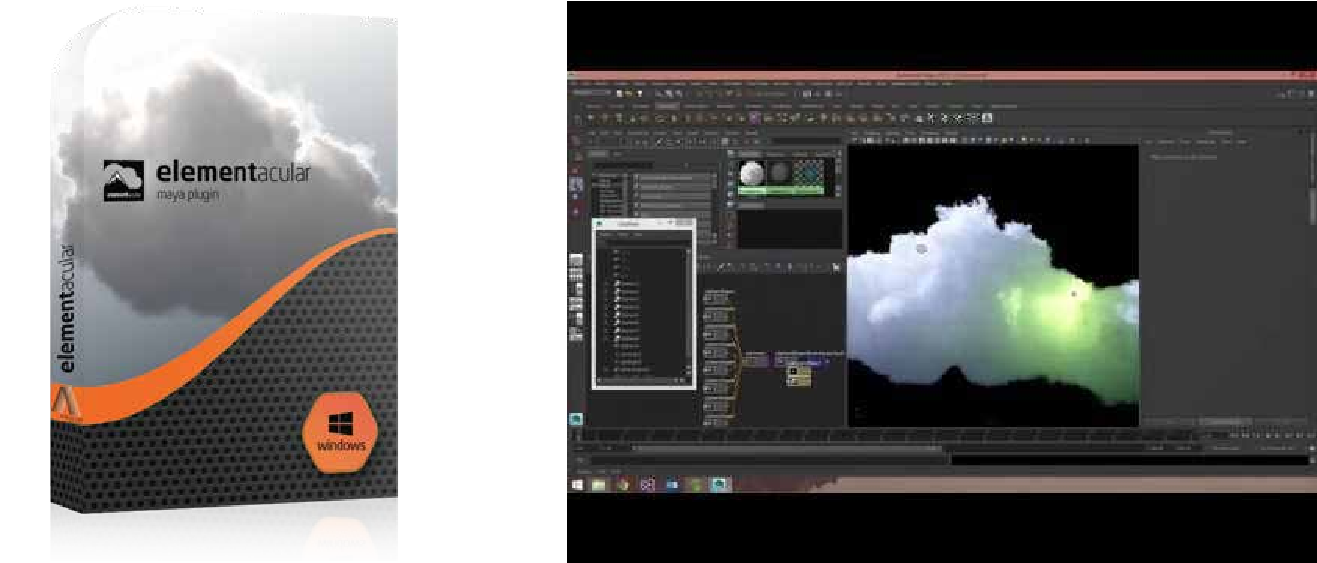
\includegraphics[width=0.95\textwidth]{07_conclusion/figures/fig_elementacular.pdf}
\caption{Flux-limited diffusion is used to compute multiple scattering in Elementacular\protect\footnotemark, a commercial plugin for interactive cloud modelling. Due to the incremental nature of interactive edits, the result from previous frames is a great initial solution for the solver, which then only needs a few iterations to resolve.}
\label{fig:fld_conclusion_elementacular_1}
\end{figure}


With $P_N$-theory, diffusion and flux-limited diffusion, this thesis gives a comprehensive treatment of the domain of deterministic methods that are based on the spherical harmonics expansion of the radiative transfer equation. For every chapter the theory is derived and a solver is being devised for solving the corresponding equations. This thesis becomes a relevant important document for understanding the methods and their application in practical applications.\footnotetext{\url{http://elementacular.com} (date of access: 10/02/2019)} 

\subsubsection*{Outlook}

However, while being comprehensive, the coverage of spherical harmonics based methods for light transport simulation in this thesis is neither exhaustive nor complete. Although it has a long history, the field is still being actively researched and advanced primarily by the nuclear science community.

The $P_N$-theory provides a solid framework for discretizing the radiative transfer equation in angular domain. However, for practical applications concerned with stead-state problems, the $P_N$-method suffers from having to solve very large linear systems if the truncation order is increased. This makes it unviable for real world applications. In addition the theory and all its derivatives, such as the diffusion approximation and flux-limited diffusion, suffer from the presence of vacuum regions in the problem domain. More specifically, all three methods will not be able to converge for these problems. This is a major issue for application in graphics, where vacuum regions are ubiquitous.

A direction for future research that has not been explored fully yet is to devise a multigrid method for solving the large coupled system of $P_N$-equations. Such a multigrid scheme could make the method more competitive in comparison to other approaches.

The introduction of the diffusion approximation has led to a variety of methods in computer graphics and a similar development can be envisioned for the $P_N$-method. The extension to finite-elements discretization or handling of more complex boundary conditions could allow the application of the $P_N$-method to problems such as subsurface scattering.

To deal with the vacuum problem one direction for future research needs to be the evaluation of the various variations of the $P_N$-method, which have been proposed in other domains, such as nuclear sciences. Evaluating these variations was one idea behind the design of the solver in chapter~\ref{sec:pnmethod}, as all the variations are presented as a coupled system of partial differential equations which could be all fed as input to the solver developed as part of this chapter.

There are no obivous open questions regarding the diffusion approximation. This comes at no surprise since diffusion has been introduced to graphics a long time ago and received a lot of attention from graphics researchers throughout the years. Its traits are known and well studied.

Flux-limited diffusion offers a great balance between computational efficiency and accuracy, therefore has seen some interest for industry application recently. As its linear counterpart, the non-linear Gauss-Seidel solver does not scale well with the resolution of the finite difference grid. Here, it seems like a promising avenue to investigate non-linear multigrid solvers. Being able to apply flux-limited diffusion to much larger problem sizes could significantly broaden its applicability.

Another interesting direction could be to extend flux-limited diffusion or even the $P_N$-theory in general to anisotropic media. All literature on $P_N$-theory is based on isotropic media and deriving a $P_N$-theory for anisotropic media could open up directions for new deterministic methods in this field. While anisotropic media appears to play a minor role in graphics at the moment, some research, such as the work by Dupuy et al.~\cite{Dupuy16}, indicates that anisotropic media might be an important building block for bridging the divide between surface rendering (rendering equation) and volume rendering (radiative transfer).

The place of deterministic methods in rendering is uncertain due to their complexities, such as discretization bias, convergence issues and boundary conditions. Particularly, deterministic methods lack the appeal of conceptional simplicity that non-deterministic methods, such as Monte-Carlo, have. This not only prevents their adoption in the industry, but also makes them unattractive as a research subject as such. This thesis represents a significant effort to fill prominent knowledge gaps and demonstrate that deterministic methods and spherical harmonics based techniques in particular can be easily understood and provide very powerful tools in rendering.







